%===============================================================================
\chapter{Turbulence and Fluid Dynamics}
\label{ch:fluids}
%===============================================================================

Fluid turbulence represents one of the most spectacular manifestations of scale hierarchy in physics. Energy injected at large scales cascades through an inertial range before being dissipated at small scales. The RG provides the natural language for describing this multi-scale structure, and this chapter applies the five-step recipe of Chapter~\ref{ch:recipe} to the Navier-Stokes and Burgers equations.

The scale hierarchy (Step 1) ranges from the integral scale $L$ of energy injection down to the Kolmogorov scale $\eta$ of viscous dissipation, with the Reynolds number measuring the separation. Coarse-graining (Step 2) integrates out velocity fluctuations at successively smaller scales while adjusting the effective viscosity. Theory space (Step 3) is parametrized by the effective viscosity and forcing spectrum. The beta functions (Step 4) describe the scale dependence of these effective parameters. Fixed-point analysis (Step 5) identifies the Kolmogorov scaling as a fixed point, with intermittency corrections arising from anomalous dimensions. Throughout, we make essential contact with Barenblatt's theory of intermediate asymptotics.

\marginnote{Turbulence involves fluctuations over a vast range of scales, making it a perfect arena for RG methods.}

%-------------------------------------------------------------------------------
\section{The Navier-Stokes Equations}
\label{sec:navier_stokes}
%-------------------------------------------------------------------------------

The incompressible Navier-Stokes equations describe the motion of a viscous fluid:
\begin{align}
\frac{\partial \mathbf{u}}{\partial t} + (\mathbf{u} \cdot \nabla)\mathbf{u} &= -\frac{1}{\rho}\nabla p + \nu \nabla^2 \mathbf{u} + \mathbf{f}, \label{eq:navier_stokes}\\
\nabla \cdot \mathbf{u} &= 0. \label{eq:incompressible}
\end{align}

Here $\mathbf{u}(\mathbf{x}, t)$ is the velocity field, $p$ the pressure, $\rho$ the density, $\nu$ the kinematic viscosity, and $\mathbf{f}$ an external forcing.

\subsection{Scale Identification}

Following Step 1 of the recipe, we identify the key scales. The integral scale $L$ characterizes the largest eddies where energy is injected, typically set by the geometry of the flow or the forcing mechanism. The Kolmogorov scale $\eta = (\nu^3/\varepsilon)^{1/4}$ characterizes the smallest eddies where viscous dissipation dominates, with $\varepsilon$ the energy dissipation rate per unit mass.

The corresponding velocity scales are the large-scale velocity $U$ at the integral scale and the Kolmogorov velocity $u_\eta = (\nu \varepsilon)^{1/4}$ at the dissipation scale. The Reynolds number $Re = UL/\nu$ measures the scale separation: for $Re \gg 1$, there is a wide inertial range $\eta \ll r \ll L$ where neither injection nor dissipation dominates. It is in this inertial range that universal scaling behavior emerges.

\marginnote{The Reynolds number is the control parameter analogous to $\rho$ in the Lorenz system or inverse temperature in statistical mechanics.}

%-------------------------------------------------------------------------------
\section{Kolmogorov Theory as an RG Fixed Point}
\label{sec:kolmogorov}
%-------------------------------------------------------------------------------

Kolmogorov's 1941 theory posits that in the inertial range, the statistics of turbulence are universal and determined only by the energy dissipation rate $\varepsilon$.

\subsection{Dimensional Analysis}

By dimensional analysis, the structure function (velocity increment moments) must scale as
\begin{equation}
S_n(r) = \langle |\mathbf{u}(\mathbf{x} + \mathbf{r}) - \mathbf{u}(\mathbf{x})|^n \rangle \sim (\varepsilon r)^{n/3}.
\label{eq:kolmogorov_scaling}
\end{equation}

This is a prediction of scale-invariant behavior, precisely what we expect at an RG fixed point (Chapter~\ref{ch:fixed_points}).

\subsection{Fixed Point Interpretation}

In the RG language, the Kolmogorov scaling~\eqref{eq:kolmogorov_scaling} corresponds to a fixed point where the effective parameters of the theory remain constant under scale change. The scaling exponent $\zeta_n = n/3$ is the analog of the scaling dimension at a CFT fixed point.

\marginnote{Deviations from K41 scaling, called intermittency corrections, indicate that the Kolmogorov fixed point is not exact.}

The RG transformation for turbulence proceeds in three stages. First, we integrate out velocity fluctuations at scales below some cutoff $\ell$, eliminating the small-scale eddies from the explicit description. Second, we rescale space by $\mathbf{x} \to s\mathbf{x}$ and velocity by $\mathbf{u} \to s^h \mathbf{u}$ where the exponent $h$ must be determined. Third, we adjust the effective viscosity to maintain the dynamical equations in their original form. At the fixed point, the effective viscosity reaches a scale-invariant value, and the scaling exponent $h = 1/3$ follows from dimensional analysis with constant $\varepsilon$.

%-------------------------------------------------------------------------------
\section{The Burgers Equation}
\label{sec:burgers}
%-------------------------------------------------------------------------------

The Burgers equation provides a simpler model that captures essential features of turbulence:
\begin{equation}
\frac{\partial u}{\partial t} + u \frac{\partial u}{\partial x} = \nu \frac{\partial^2 u}{\partial x^2}.
\label{eq:burgers}
\end{equation}

\subsection{Self-Similar Solutions}

The Burgers equation admits self-similar solutions of the form
\begin{equation}
u(x, t) = t^{-\alpha} f(\xi), \quad \xi = x/t^\beta
\end{equation}
where $\alpha$ and $\beta$ are scaling exponents determined by requiring that the similarity ansatz solve the equation.

\marginnote{Self-similar solutions are the hallmark of intermediate asymptotics, describing behavior far from both initial conditions and final equilibrium.}

Substituting into~\eqref{eq:burgers} gives constraints on the exponents. For the inviscid limit $\nu \to 0$, we find $\alpha = \beta = 1/2$ (first kind self-similarity). With viscosity, anomalous dimensions can appear.

\subsection{Connection to Intermediate Asymptotics}

Following Barenblatt \cite{Barenblatt1979}, self-similar solutions arise in the ``intermediate asymptotic'' regime where the solution has forgotten initial conditions but has not yet reached final equilibrium.

The RG interpretation is direct: intermediate asymptotics corresponds to the RG flow approaching a fixed point. The self-similar exponents are scaling dimensions at this fixed point. First-kind similarity (where exponents follow from dimensional analysis) corresponds to a classical fixed point, while second-kind similarity (with anomalous exponents) corresponds to a nontrivial quantum/fluctuation-corrected fixed point.

%-------------------------------------------------------------------------------
\section{RG for Navier-Stokes}
\label{sec:ns_rg}
%-------------------------------------------------------------------------------

Several approaches apply RG to the Navier-Stokes equations.

\subsection{Yakhot-Orszag $\varepsilon$-Expansion}

Inspired by the Wilson-Fisher $\varepsilon$-expansion for critical phenomena (Chapter~\ref{ch:on_model}), Yakhot and Orszag developed an RG approach to forced Navier-Stokes turbulence. Their key insight was that the forcing power spectrum provides a tunable parameter analogous to $\varepsilon = 4 - d$ in scalar field theory.

The forcing is taken to have power-law spectrum $\sim k^{y}$ where $y$ is varied as a control parameter (analogous to $\varepsilon = 4 - D$ in $\phi^4$ theory). The RG flow equations for the effective viscosity $\nu$ and forcing amplitude $D_0$ are:
\begin{align}
\frac{\dd \nu}{\dd s} &= \nu \left[ z - 2 + \frac{A D_0}{\nu^3} + \cdots \right], \\
\frac{\dd D_0}{\dd s} &= D_0 \left[ y + 4 - 2z + \cdots \right],
\end{align}
where $z$ is the dynamic exponent and $A$ is a calculable constant.

At the fixed point, these equations give Kolmogorov-like scaling with computable corrections.

\begin{workedbox}[Box 10.1: Derivation of the Yakhot-Orszag Beta Functions]
\textbf{Setup:} The Navier-Stokes equation in Fourier space with random forcing $\mathbf{f}$ having correlation $\langle f_i(\mathbf{k}) f_j(\mathbf{k}') \rangle = D_0 k^y P_{ij}(\mathbf{k}) \delta(\mathbf{k} + \mathbf{k}')$, where $P_{ij}$ is the transverse projector.

\textbf{Step 1 (Dimensional analysis):} The viscosity has dimensions $[\nu] = L^2/T$, so $\nu$ scales as $\ell^{2-z}$ under $x \to \ell x$, $t \to \ell^z t$. The forcing amplitude has $[D_0] = L^{4-y}/T^3$, so $D_0 \to \ell^{4-y-2z}D_0$.

\textbf{Step 2 (Coarse-graining):} Integrate out velocity modes with $|\mathbf{k}| > \Lambda/b$ where $b > 1$. The key one-loop diagram is:
\begin{equation}
\vcenter{\hbox{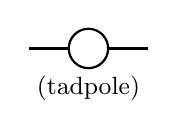
\begin{tikzpicture}[scale=0.5]
\draw[thick] (-1.5,0) -- (-0.5,0);
\draw[thick] (0.5,0) -- (1.5,0);
\draw[thick] (0,0) circle (0.5);
\node at (0,-1) {\small (tadpole)};
\end{tikzpicture}}}
\end{equation}

\textbf{Step 3 (Loop integral):} The one-loop correction to the effective viscosity is:
\begin{equation}
\delta\nu = -A \int_{\Lambda/b}^{\Lambda} \frac{d^d k}{(2\pi)^d} \frac{D_0 k^y}{k^2 \cdot (k^2 + \nu k^2)^2} \approx \frac{A D_0 \Lambda^{y-2}}{\nu^2} \ln b
\end{equation}
where $A$ is a geometric factor from the angular integration.

\textbf{Step 4 (Beta functions):} Taking $b = e^{ds}$ and combining with dimensional scaling:
\begin{align}
\beta_\nu &= (z-2)\nu + \frac{A D_0}{\nu^2 \Lambda^{2-y}} \\
\beta_{D_0} &= (y + 4 - 2z)D_0
\end{align}

\textbf{Fixed point:} Setting $\beta_{D_0} = 0$ determines $z = (y+4)/2$. For Kolmogorov turbulence with constant energy flux, $y = 4$ gives $z = 4$, which is modified by the viscosity correction to yield $z \approx 2$ (the Kolmogorov result $u \sim r^{1/3}$ comes from $h = 1/z$).

\textbf{Physical interpretation:} The fixed point represents the balance between energy injection at large scales and dissipation at small scales. The anomalous corrections come from the nonlinear mode coupling.
\end{workedbox}

\subsection{Functional RG}

The functional RG approach can also be applied to turbulence. This nonperturbative method defines an effective action $\Gamma_k[\mathbf{u}]$ that incorporates fluctuations at scales larger than $1/k$. The Wetterich equation describes its flow:
\begin{equation}
\frac{\partial \Gamma_k}{\partial s} = \frac{1}{2} \mathrm{Tr} \left[ \left( \Gamma_k^{(2)} + R_k \right)^{-1} \frac{\partial R_k}{\partial s} \right]
\end{equation}
where $s = \ln(k_0/k)$ and $R_k$ is the regulator.

\marginnote{The functional RG provides a nonperturbative approach that can handle strong fluctuations.}

%-------------------------------------------------------------------------------
\section{Energy Cascade and Irreversibility}
\label{sec:cascade}
%-------------------------------------------------------------------------------

Turbulence exhibits a characteristic irreversible flow of energy from large to small scales.

\subsection{Energy Flux}

In the inertial range, energy is transferred from scale to scale at a constant rate $\varepsilon$. This cascade is described by the K\'arm\'an-Howarth equation:
\begin{equation}
\frac{\partial}{\partial t}\langle u^2 \rangle = -\frac{2}{r}\frac{\partial}{\partial r}(r^2 \varepsilon_r) + 2\nu \nabla^2 \langle u^2 \rangle
\end{equation}
where $\varepsilon_r$ is the energy flux at scale $r$.

\subsection{Connection to the c-Theorem}

The monotonic decrease of energy to small scales is analogous to the c-theorem in conformal field theory. We can define an ``enstrophy'' (mean-square vorticity in 2D) or other quantities that decrease monotonically along the RG flow.

\marginnote{The energy cascade implements irreversibility in turbulence, just as the c-function decrease implements irreversibility in QFT.}

In 2D turbulence, there is additionally an inverse cascade of energy to large scales, while enstrophy cascades to small scales. This dual cascade structure reflects the additional conserved quantity in 2D.

%-------------------------------------------------------------------------------
\section{Intermittency and Anomalous Dimensions}
\label{sec:intermittency}
%-------------------------------------------------------------------------------

Experimental measurements show systematic deviations from K41 scaling:
\begin{equation}
S_n(r) \sim r^{\zeta_n}, \quad \zeta_n \neq n/3.
\end{equation}

These deviations, called intermittency, indicate that the simple Kolmogorov fixed point does not capture the full physics.

\subsection{Multifractal Models}

The deviation $\Delta_n = \zeta_n - n/3$ represents anomalous dimensions arising from the multi-scale structure of dissipation. Various phenomenological models (log-normal, She-Leveque, etc.) parameterize these corrections.

\marginnote{Intermittency corrections are the turbulent analog of anomalous dimensions in critical phenomena.}

\subsection{RG Interpretation}

From the RG viewpoint, intermittency arises because the Kolmogorov fixed point has relevant or marginally relevant perturbations. The flow does not exactly reach the fixed point, and corrections to scaling appear.

This is analogous to the situation in $\phi^4$ theory where the Wilson-Fisher fixed point has corrections from irrelevant operators that give subleading scaling behavior.

%-------------------------------------------------------------------------------
\section{Application: Shock Waves in Burgers}
\label{sec:shock}
%-------------------------------------------------------------------------------

As a concrete application, consider shock formation in the inviscid Burgers equation.

\subsection{Method of Characteristics}

The inviscid Burgers equation $u_t + uu_x = 0$ can be solved by characteristics. For smooth initial data $u(x, 0) = u_0(x)$, the solution develops shocks in finite time when characteristics cross.

\subsection{Intermediate Asymptotics}

After shock formation, the solution enters an intermediate asymptotic regime where the specific initial conditions are forgotten but the overall structure of shocks persists.

The similarity solution for a single shock is
\begin{equation}
u(x, t) = \frac{x}{t}
\end{equation}
for $|x| < s(t)$ where $s(t)$ is the shock position. This is a self-similar solution of the first kind.

\subsection{Viscous Corrections}

With small viscosity $\nu > 0$, the shock has finite width $\sim \nu/\Delta u$ where $\Delta u$ is the velocity jump. The shock structure is
\begin{equation}
u(x, t) = \frac{u_L + u_R}{2} - \frac{\Delta u}{2}\tanh\left(\frac{\Delta u (x - st)}{4\nu}\right)
\end{equation}
where $u_L, u_R$ are the velocities on either side and $s = (u_L + u_R)/2$ is the shock speed.

\marginnote{The shock width $\sim \nu$ is the dissipation scale, analogous to the Kolmogorov scale $\eta$ in turbulence.}

This solution illustrates how small-scale physics (viscosity) regularizes the large-scale dynamics (shock), precisely the multi-scale structure that the RG is designed to handle.

%-------------------------------------------------------------------------------
\section{Connection to the Geometric Framework}
\label{sec:fluids_geometry}
%-------------------------------------------------------------------------------

We now make explicit the connection to Part I.

\subsection{Theory Space for Fluids}

The couplings that parametrize theory space for fluid dynamics include the viscosity $\nu$ (or equivalently the Reynolds number $Re$), parameters characterizing the forcing spectrum such as its amplitude and spatial structure, and any additional dimensionless parameters that enter the problem. For homogeneous isotropic turbulence with power-law forcing, the essential parameters reduce to the effective viscosity and the forcing exponent.

The RG flow describes how the effective viscosity changes as we coarse-grain:
\begin{equation}
\frac{\dd \nu_{\text{eff}}}{\dd s} = \beta_\nu(\nu_{\text{eff}}, \ldots).
\end{equation}
At the Kolmogorov fixed point, $\beta_\nu = 0$ and the effective viscosity has reached a scale-invariant value. The fixed-point theory describes the universal scaling behavior in the inertial range.

\subsection{Self-Similarity from Equivariance}

The self-similar solutions of Section~\ref{sec:burgers} arise from the scale covariance requirement discussed in Chapter~\ref{ch:rg_equation}. If the solution is to be independent of the arbitrary choice of length scale, it must take the self-similar form.

The scaling exponents emerge as eigenvalues of the RG transformation, exactly as in Chapter~\ref{ch:fixed_points}.

%-------------------------------------------------------------------------------
\section{Summary}
\label{sec:fluids_summary}
%-------------------------------------------------------------------------------

This chapter has applied the five-step RG recipe to turbulence and fluid dynamics. The scale hierarchy (Step 1) spans from the integral scale $L$ to the Kolmogorov scale $\eta$, with the Reynolds number measuring the separation. Coarse-graining (Step 2) integrates out velocity fluctuations while rescaling space and adjusting the effective viscosity. Theory space (Step 3) is parametrized by the effective viscosity and forcing spectrum. The beta functions (Step 4) from the Yakhot-Orszag analysis describe the scale dependence of these effective parameters. Fixed-point analysis (Step 5) identifies Kolmogorov scaling as a fixed point.

The RG perspective reveals Kolmogorov scaling as fixed-point behavior, with structure function exponents playing the role of scaling dimensions. Intermittency corrections are anomalous dimensions arising from the multi-scale structure of dissipation. Self-similar solutions of the Burgers equation exemplify fixed-point structure in its simplest form. The energy cascade, transferring energy monotonically from large to small scales, is an irreversible RG flow analogous to the $c$-theorem in two-dimensional field theory. Barenblatt's intermediate asymptotics provides the physical interpretation of approach to a fixed point.

This chapter demonstrates that the geometric RG framework unifies the treatment of turbulence with critical phenomena, revealing the deep mathematical connections between fluid dynamics and statistical physics. The same five-step recipe that organized the anharmonic oscillator and Lorenz equations applies equally well to the Navier-Stokes equations, despite the enormous increase in complexity.

